\documentclass[class=article,border=0pt]{standalone}
\usepackage{fancybox,pstricks,pst-node,tikz}
\usetikzlibrary{decorations.markings}
\usetikzlibrary{patterns}

\newcommand*{\xMin}{-10}%
\newcommand*{\xMax}{3}%
\newcommand*{\yMin}{-3}%
\newcommand*{\yMax}{1}%
\begin{document}

\pagestyle{empty}%
\thispagestyle{empty}%
\psset{linewidth=1.5pt,framearc=0.3}%
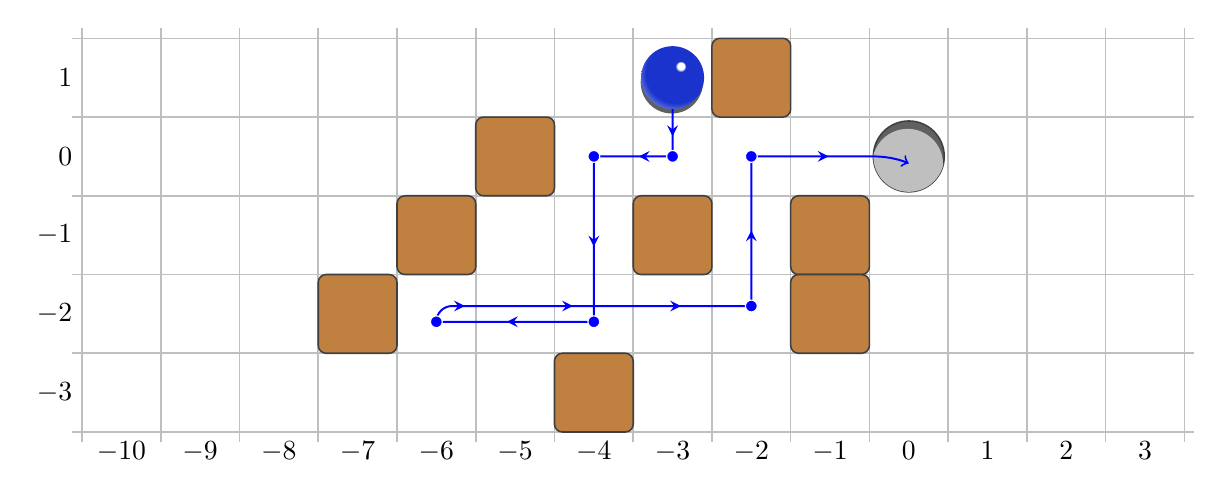
\begin{tikzpicture}

% Grid
\foreach \i in {\xMin,...,\xMax} {
  \draw [draw=none] (\i,\yMin) -- (\i,\yMax)  node [below] at (\i+0.5,\yMin) {$\i$};
}
\foreach \i in {\yMin,...,\yMax} {
   \draw [draw=none] (\xMin,\i) -- (\xMax,\i) node [left] at (\xMin,\i+0.5) {$\i$};
}
\draw[step=10mm, line width=0.2mm, black!25]
  (\xMin-0.125,\yMin-0.125) grid (\xMax+1.125,\yMax+1.125);

% Centre hole
\draw [draw=black!75,fill=black!62.5,line width=0.2mm] (0.5,0.5) circle (.45);
\begin{scope}
  \clip [draw=none] (0.485,0.4) circle (.45);
  \draw [draw=none,fill=black!25,line width=0.2mm] (0.5,0.5) circle (.45);
\end{scope}

% Marble
\pgfdeclareradialshading{marble}{\pgfpoint{0.25cm}{0.35cm}}{%
  rgb(0cm)=(1,1,1);
  rgb(0.10cm)=(1,1,1);
  rgb(0.15cm)=(0.1,0.2,0.8);
  rgb(0.85cm)=(0.1,0.2,0.8);
  rgb(1.4cm)=(1,1,1)
}
\draw[fill=black!62.5,draw=none] (-2.51, 1.44) circle (0.395);
\draw[draw=none,shading=marble] (-2.5, 1.5) circle (0.4);

% Blocks
\begin{scope}[
    rounded corners=1mm,
    line width=0.2mm
  ]
  \filldraw [brown,draw=black!75] (-1,-1) rectangle++(1,1);
  \filldraw [brown,draw=black!75] (-1,-2) rectangle++(1,1);
  \filldraw [brown,draw=black!75] (-2, 1) rectangle++(1,1);
  \filldraw [brown,draw=black!75] (-3,-1) rectangle++(1,1);
  \filldraw [brown,draw=black!75] (-5, 0) rectangle++(1,1);
  \filldraw [brown,draw=black!75] (-6,-1) rectangle++(1,1);
  \filldraw [brown,draw=black!75] (-7,-2) rectangle++(1,1);
  \filldraw [brown,draw=black!75] (-4,-3) rectangle++(1,1);
\end{scope}

% Route taken
\begin{scope}[
  very thick,
  decoration={
    markings,
    mark=at position 0.025 with {\arrow{stealth}},
    mark=at position 0.075 with {\arrow{stealth}},
    mark=at position 0.200 with {\arrow{stealth}},
    mark=at position 0.350 with {\arrow{stealth}},
    mark=at position 0.450 with {\arrow{stealth}},
    mark=at position 0.550 with {\arrow{stealth}},
    mark=at position 0.650 with {\arrow{stealth}},
    mark=at position 0.785 with {\arrow{stealth}},
    mark=at position 0.925 with {\arrow{stealth}},
  }]
  \draw[line width=0.25mm,->,blue,postaction={decorate}]
       (-2.5,  1.1)
    -- (-2.5,  0.5)
    -- (-3.5,  0.5)
    -- (-3.5, -1.6)
    -- (-5.5, -1.6) arc(-180:-270:0.2)
    -- (-5.3, -1.4)
    -- (-1.5, -1.4)
    -- (-1.5,  0.5)
        % Falling into the hole.
        -- (0.05, 0.5)
        arc(90:68:1.2);
\end{scope}

% Collision points.
\draw [fill=blue,draw=white] (-2.5,  0.5) circle (0.075);
\draw [fill=blue,draw=white] (-3.5,  0.5) circle (0.075);
\draw [fill=blue,draw=white] (-3.5, -1.6) circle (0.075);
\draw [fill=blue,draw=white] (-5.5, -1.6) circle (0.075);
\draw [fill=blue,draw=white] (-1.5, -1.4) circle (0.075);
\draw [fill=blue,draw=white] (-1.5,  0.5) circle (0.075);


\end{tikzpicture}


\end{document}
